\documentclass{report}

\usepackage{tikz}
\usetikzlibrary{shapes}

\usepackage{subcaption}

\newcommand{\ie}{{\textit{i.e.\ }}}
\newcommand{\cf}{{\textit{cf\ }}}
\newcommand{\eg}{{\textit{e.g.\ }}}
\newcommand{\al}{{\textit{et al.\ }}}


\begin{document}

\title{Mutual Modeling in Human-Robot Interaction - Scientific part}

\chapter{Scientific Part}
\section{Summary}

\paragraph{Mutual Modelling}

In order to build a shared understanding, do partners have to build a
representation of each other's knowledge? We refer to \emph{mutual modeling} (MM) as
the process of inferring one's partner mental states. Any claim that students
carry out a detailed monitoring of their peers would be as incorrect as any
claim that they do not maintain any representation at all. If mutual modeling
had to be permanently detailed and accurate, subjects would obviously face a
huge cognitive load. Conversely, peers could not collaborate without some
minimal amount of mutual modeling. For instance, A cannot disagree with B
without knowing that B has a different opinion. The mutual model can be implicit
(A is not aware of what he knows about B), by-default (I believe that B beliefs
what I believe unless contrary evidence), opportunistic (A does not model B
unless the conversation requires it), global (A infers B's beliefs based on
categories such as age, culture or profession) and, of course, it can be
incorrect… but it can not remain empty. Dialogues include many instances of
utterances such as "I thought he would do that" (first level of MM) or even "He
thought I would do that but I intended something else." (second level of MM). 

The content of mutual models ranges from 'dispositional' versus 'situational'
aspects. The 'dispositional' aspects refer to A's representation of B's long
term knowledge, skills or traits. It is thus closely related to the notion of
transactive memory (Wegner, 1987; Moreland, 2000). 'Situational' aspects refer
to A's representation of B's knowledge, behavior or intentions specifically
activated in the situation in which A and B are collaborating, some of them
being valid for 2 seconds, other ones for 2 hours. Here are examples of
fragments that constitute A's model of B regarding to aspects X, noted
$Model(A,B,X)$:

\begin{itemize}

    \item $Model(A,B, knowledge)$: What does A know about B's knowledge with
        respect to the task at hand or, inversely, about B's knowledge gaps?
        When can A consider B's statements as reliable? 

    \item $Model(A,B, skills)$: What does A know about B's skills with respect to
        the task at hand? May A expect B to perform well in a specific subtask?
        The effectiveness of division of labor depends on the quality of this
        mutual model. 

    \item $Model(A,B, goals)$: What does A know about B's intentions with respect
        to the project, including B' motivation and commitment? Can A trust B
        when B promises to deliver? 

    \item $Model(A,B, task)$: What does A know about B's representation of the
        situation and the task: does A knows whether B has the same
        understanding of the problem at stake? 

    \item $Model(A,B, plans)$: What does A know about B's strategy. Does A
        understand why B did what he did? Is A able to anticipate what B will do
        next? 

    \item $Model(A,B, "urgent")$: What does A about know B's understanding of A's
        last utterance: does ‘urgent’ means now, ASAP and ‘not too lat’ ?

    \item We could continue the list of what is X is $\mathcal{M}(A,B,X)$: beliefs,
        emotions, history, status, …

\end{itemize}

We have different levels of MM. If A states "B thinks I am god in maths", we
are the second level of MM:  $Model(A, B, Model(B,A, knowledge="good in
math"))$. There is an infinite regress of nested models: If A says "B knows that
I don't expect him to solve this statistics problem" corresponds to $Model(A, B,
Model (B, A (Model (A,B, statistic-skills)))$.

A partner model is probably not a "box", \ie not a monolithical representation
but rather a mosaic of information fragments about the partner, with various
grain sizes and various life cycles. This mosaic is elaborated through various
mechanisms, first for building an initial model of the partner and then for
updating this model.  As two students meet for the first time, mutual models are
initialized by the assumptions they make upon each other from cues such as
his/her membership to large categories (age, culture, profession, ...) include
stereotypes (sportsmen, junkie, business women, Swiss,…) as well as physical
appearance. Scholars studied how initial modeling impacts communication. In
their experiments on initial MM, Slugoski, Lalljee, Lamb \& Ginsburg (1993)
pretended to their subjects that their (fake) partner had or had not received
the same information. They observed that the subjects adapted their dialogue by
focusing the explanation on the items that (s)he was supposed to ignore. Brennan
(1991) showed that the subjects used different initial strategies in forming
queries depending on who they were told their partner was.  

Initial common grounds are also initiated by co-presence: they include events to
which A and B attended together (Clark \& Marshall, 1981) in the physical space
or in our cultural space (\eg ‘09-11’). Co-presence means that we can refer to
a shared objects and event,-s it does of course not imply that we give them the
same meaning. Namely, a shared screen does not mean a shared understanding
(Dillenbourg \& Traum, 2006).

After initialization, mutual models are updated along the collaborative work
through verbal and non-verbal interactions. A default inference rule is that "my
partner agrees with me unless he disagrees", which reject the critiques that
mutual modeling generates an unbearable cognitive load. This default rule is
superseded by the several mechanisms for monitoring and repairing one's partner
understanding: acknowledgement, continuous attention, relevance of next turns,
facial expressions including gaze signals, etc.

Mutual modeling does not occur in a vacuum but it is highly contextualized. REF
reviews the features of the collaborative situation, namely the media
(cotemporality… ), may facilitate or hamper mutual modeling. Hutchins (SILENCE)
reported a study in which a short silence between two pilots was perfectly
interpreted because it occurred in a highly constrained communication context.
Some environments are more productive than others in helping peers to detect
their misunderstandings. Roschelle (REF) reformulate the design of CSCL
interfaces as providing ways for peer to detect and repairs their
misunderstanding. In CSCW, researchers have explored various so-called
"awareness tools", \ie functionalities that inform A is about B's actions that
A could not directly perceived because B was working on a different subset of
the virtual space. Different awareness tools will be addressed in this
contribution since they allowed us to manipulate experimentally the MM activity. 

\section{Research Plan}

\subsection{State of the Art}

\subsection{Related research of the requirers}

\subsection{Detailed research plan}

\subsubsection{Simple model of mutual modeling}

To report experiments on MM, we use a simple notational system: "A knows that B
knows X", noted $\mathcal{M}(A,B,X)$ is a simplistic but hopefully useful reduction to
reason on mutual modeling. This notation does not mean A as an explicit,
monolithic representation of B: It is an abstraction referring to complex
socio-cognitive processes. 

We refer to the degree of accuracy of the mutual model as
$\mathcal{M}^{\circ}(A,B,X)$. To estimate, the MM effort, we need 3 variables. 

\begin{enumerate}
    
    \item Tasks vary a lot with respect to how much they require.  The grounding
        criterion – denoted $\mathcal{M}^{\circ}_{min}$  - refers to how
        important it is to mutually share a piece of information X to succeed
        the task T.. It can be computed as the probability to succeed T despite
        the fact X is not grounded. In the next studies, we estimate
        $\mathcal{M}^{\circ}_{min}(A,B,X)$ as the correlation between
        $\mathcal{M}^{\circ}(A,B,X)$ and task performance. 

    \item Before any specific grounding act, there is rarely a null probability
        that X is mutually understood by A and B: because X is part of A's and
        B's cultures, because it is manifest to co-present subjects or simply
        because there is not much space for misunderstanding or disagreement
        about X. We could not simply collaborate without a high level of initial
        grounds. We note the theoretical accuracy of initial grounds:
        $\mathcal{M}^{\circ}_{t1}(A,B,X)$.

    \item The cost of grounding X refers to the physical and cognitive effort
        necessary to perform a grounding act α: a verbal repair (\eg
        rephrasing), a deictic gesture, a physical move to adopt one partner's
        viewpoint, etc. This cost varies according to media features ( Clark \&
        Brennan (REF….). 

\end{enumerate}

Based on these 3 parameters, the probability of making an action $\alpha_{t1}$ about
content X at time $t1$ during task T for increasing $\mathcal{M}^{\circ}(A,B,X)$
at time $t2$ is the ratio between how much it is needed  ((2)-(1)) and how much it
costs (3)(Traum \& Dillenbourg, 1996):

$p(\alpha_{t1}(X,T)   M^{\circ}_{t2}(A,B,X)) ≈ (M^{\circ}_{min}(A,B,X,T) -
M^{\circ}_{t1}(A,B,X))/cost (\alpha)$

This is qualitative summary more that a real equation since several parameters
are hard to quantify (\eg the cost an communication acts depends upon the user
as well) but it clarifies the parameters of the experiments we report hereafter.

\begin{itemize}
    \item $\mathcal{M}^{\circ}(A,B,X)$: Our experiments address different contents that can be
        represented in mutual models:

        \begin{enumerate}
            \item $\mathcal{M}(A,B,emotion)$: how accurately A perceives B's emotional state
                (study 3); 

            \item $\mathcal{M}(A,B,actions)$ is about how well A guesses what action B has
                done (study 2) or will do next  (study 1)

            \item $\mathcal{M} (A,B,knowledge)$: how accurately A estimates B's knowledge
                with respect to the material they learn together (study 4 and 5)

        \end{enumerate}

    \item $\mathcal{M}^{\circ\circ}(A,B,X,T)$ Our studies concern various collaborative tasks:
        argumentation (study 3), games (study 1 and 2) and concept mapping
        (study 4 and 5). By varying the tasks, we do actually vary the grounding
        criterion but they all require a "reasonably high" grounding criterion.
        All tasks are about building a solution or a representation together; we
        did not address everyday conversations. 

    \item $\mathcal{M}^{\circ}_{t1}(A,B,X)$ Along the same reasoning, the initial degree
        of common grounds should be rather low (and hence the difference between
        initial and required degrees rather high) in order to make mutual
        modelling effort more observable. Studies 1, 4 and 5 have been conducted
        with teams of students who did not know each other. They came
        nonetheless from the same university: they hence had some general common
        grounds.  For studies 2 and 3, students knew each other before for
        reasons explained later on. In study 5, we manipulated the initial MM by
        using a JIGSAW script.

    \item $cost(\alpha)$ In all studies but study 4, the cost of  grounding is
        an independent variable. Study 3 uses media richness as independent
        variable, with the hypothesis that modeling emotions is "cheaper" with a
        richer medium, \ie  when peers can see each other.  Studies 1,2 and 4
        use awareness tools which, in principle, reduce the cost of MM, but do
        not eliminate all costs: if the tool provide A with information about
        what B does/knows, this additional information may actually increase
        cognitive load. Awareness tools constitute as a kind of MM prosthesis,
        and, like any prosthesis, they many augment MM (by facilitating it or
        even scaffolding it) or inhibit it (by making it useless).

\end{itemize}


Measuring $\mathcal{M}^{\circ}(A,B,X)$ is methodologically difficult. We
discriminate two steps, first to capture $\mathcal{M}(A,B,X)$ and then to
estimate $\mathcal{M}^{\circ}(A,B,X)$. 

\begin{itemize}
    \item Capturing M (A,B,X) The simplest method is to ask A what (s)he
        believes about what B knows, feels, intends to do, etc. This raises
        obvious methodological concerns since such a question triggers a
        modeling process beyond what it would 'naturally' be. To avoid this
        bias, one can estimate mutual modeling after task completion. Then, the
        obvious drawback are memory losses and by post-hoc reconstruction. We
        have no other choice:. The first method was used in study 2 and the
        second one in the other studies.  

    \item Estimating $\mathcal{M}^{\circ}(A,B,X)$. The accuracy of
        $\mathcal{M}(A,B,X)$ can be
        estimated in 2 ways.
        \begin{itemize}
            \item Subjective accuracy: In study 3, we compute
                $\mathcal{M}^{\circ}(A,B,emotions)$ by measuring if A describe
                B's emotions in the same way B reports her emotions (
                ($\mathcal{M}(A,B)=\mathcal{M}(B,B)$) 
                
            \item Objective accuracy: In studies 4 and 5, w we compute
                $\mathcal{M}^{\circ}(A,B,knowledge)$ by comparing
                $\mathcal{M}^{\circ}A,B,K)$ to B's actual knowledge as it has
                measured by a test. 

        \end{itemize}

\end{itemize}

\subsubsection{Research questions}

The experiments we report here address MM across different tasks, some with
dyads, other with triads. They were conducted along 6 years in two different
institutions by different researchers. They used different independent,
intermediate and dependent variables. Nonetheless, we were able to address a few
questions across these studies. We start with 3 simple hypotheses about
$\mathcal{M}^{\circ}(A,B)$:

\begin{itemize}
    \item $\mathcal{H}_{1}$: $\mathcal{M}^{\circ}(A,B)$ depends upon A’s ability or effort
        to model B,
    
    \item $\mathcal{H}_{2}$: $\mathcal{M}^{\circ}(A,B)$ depends upon  B’s ability of
        effort to help A to model him/herself 

    \item $\mathcal{H}_{3}$: $\mathcal{M}^{\circ}(A,B)$ depends upon the quality of
        interactions among A and B

\end{itemize}



$\mathcal{H}_{2}$ is also called a second level modeling hypothesis since H
needs to monitor B to see if A understood him/her
$\mathcal{M}(B,(A,\mathcal{M}(A,B)))$

Our main issue is the symmetry questions: what is the relationship (fig.1)
between $\mathcal{M}^{\circ}(A,B,X)$ and $\mathcal{M}^{\circ}(B,A,X)$? A low
symmetry would mean that mutual modeling
is mainly an individual attitude/aptitude ($\mathcal{H}_{1}$). A high
correlation might support $\mathcal{H}_{2}$ since there is a low probability
that randomly formed pairs integrate peers with the same level of MM skills.

\begin{figure*}[htb]
\centering

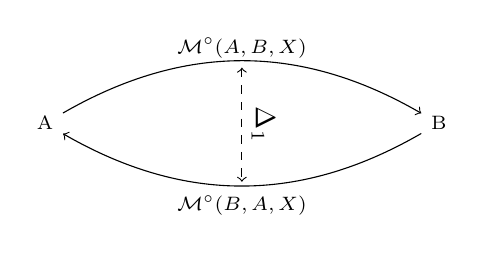
\begin{tikzpicture}[scale=0.5]

\draw(0,0) node[anchor=north] (A) {\scriptsize A};
\draw(10,0) node[anchor=north] (B) {\scriptsize B};
\draw(5,2) node[anchor=north] {\scriptsize $\mathcal{M}^{\circ}(A, B, X)$};
\draw(5,-2) node[anchor=north] {\scriptsize $\mathcal{M}^{\circ}(B, A, X)$};
\draw[dashed, <->] (5,1) -- (5,-1.9) node[midway, sloped, above] {$\Delta_1$};
\draw[->] (A) to[bend left] (B);
\draw[->] (B) to[bend left] (A);

\end{tikzpicture}

\caption{The MM symmetry question $\Delta_1 =  \Delta(\mathcal{M}^{\circ} (A,B,X),
\mathcal{M}^{\circ} (B,A,X))$}

\label{mm_symetry}
\end{figure*}


With triads, we may compute the accuracy of 6 models:
$\mathcal{M}^{\circ}(A,B)$, $\mathcal{M}^{\circ}(B,A)$,
$\mathcal{M}^{\circ}(A,C)$, $\mathcal{M}^{\circ}(C,A)$,
$\mathcal{M}^{\circ}(C,B)$ and $\mathcal{M}^{\circ}(B,C)$. This enables two
triangle questions (see figure 2):

Do A and B have the same accuracy when modeling C? $\Delta2 =
\Delta(\mathcal{M}(A,C,X), \mathcal{M}(B,C,X))$ If it is the same,
$\mathcal{H}_{2}$ and $\mathcal{H}_{3}$ gain over $\mathcal{H}_{1}$

Does C model more accurately A than B? $\Delta3= \Delta(\mathcal{M}(C,A,X),
\mathcal{M}(C,B,X))$ A positive answer would support $\mathcal{H}_{3}$.

\begin{figure}[htb]
\centering
\subcaptionbox{}{ 
    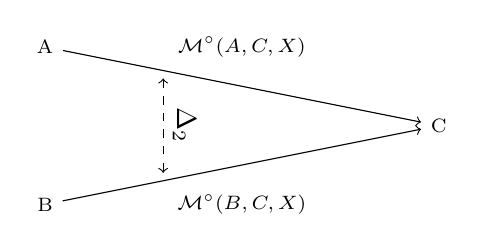
\begin{tikzpicture}[scale=0.5]

    \draw(0,2) node (A) {\scriptsize A};
    \draw(0,-2) node (B) {\scriptsize B};
    \draw(10,0) node (C) {\scriptsize C};

    \draw(5,2) node {\scriptsize $\mathcal{M}^{\circ}(A, C, X)$};
    \draw(5,-2) node {\scriptsize $\mathcal{M}^{\circ}(B, C, X)$};
    \draw[dashed, <->] (3,1.2) -- (3,-1.2) node[midway, sloped, above] {$\Delta_2$};
    \draw[->] (A) to (C);
    \draw[->] (B) to (C);

    \end{tikzpicture}
}
\subcaptionbox{}{ 
    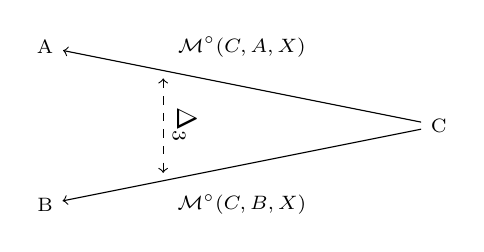
\begin{tikzpicture}[scale=0.5]

    \draw(0,2) node (A) {\scriptsize A};
    \draw(0,-2) node (B) {\scriptsize B};
    \draw(10,0) node (C) {\scriptsize C};

    \draw(5,2) node {\scriptsize $\mathcal{M}^{\circ}(C, A, X)$};
    \draw(5,-2) node {\scriptsize $\mathcal{M}^{\circ}(C, B, X)$};
    \draw[dashed, <->] (3,1.2) -- (3,-1.2) node[midway, sloped, above]
    {$\Delta_3$};
    \draw[<-] (A) to (C);
    \draw[<-] (B) to (C);

    \end{tikzpicture}
}
\caption{The MM triangle questions}

\label{mm_triangle}
\end{figure}



In addition, the comparison between ($\Delta2$) and ($\Delta3$) could tell us
whether the accuracy of mutual modelling depends more upon the modeller's effort
or the modellee's behaviour.

The rectangle questions 

We could go further by comparing self- versus other modeling ($\Delta4$ in Fig.
3) as an indication of metacognitive skills. We could also see if modeling
skills depend upon what aspects are being modeled (X or Y), which would explain
vertical differences ($\Delta5$ in Fig. 3). We do not further develop these
questions because we don’t have the necessary data in our studies.

\begin{figure*}[htb]
\centering

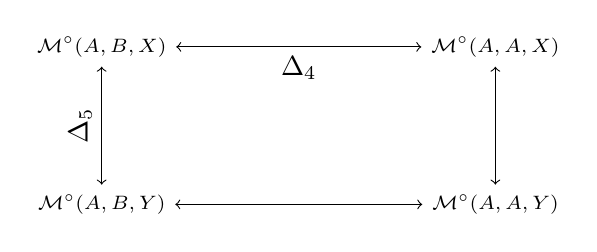
\begin{tikzpicture}[scale=0.5]

    \draw(0,0) node (a) {\scriptsize $\mathcal{M}^{\circ}(A, B, X)$};
    \draw(10,0) node (b) {\scriptsize $\mathcal{M}^{\circ}(A, A, X)$};
    \draw(10,-4) node (c) {\scriptsize $\mathcal{M}^{\circ}(A, A, Y)$};
    \draw(0,-4) node (d) {\scriptsize $\mathcal{M}^{\circ}(A, B, Y)$};
    \draw[<->] (a) -- (b) node[midway, below] {$\Delta_4$};
    \draw[<->] (b) -- (c);
    \draw[<->] (c) -- (d);
    \draw[<->] (d) -- (a) node[midway, sloped, above] {$\Delta_5$};

\end{tikzpicture}

\caption{The rectangle questions}

\label{mm_rectangle}
\end{figure*}


This simple notation does not pretend to provide a mathematical account of
mutual modeling but to be more systematic in describing the following
experiments. 

\subsection{Research agenda}

\subsection{Importance of the work}

\subsection{References}

\section{International collaboration}

\end{document}

